\chapter{Hankow}

\begin{figure}[htbp]
\centering
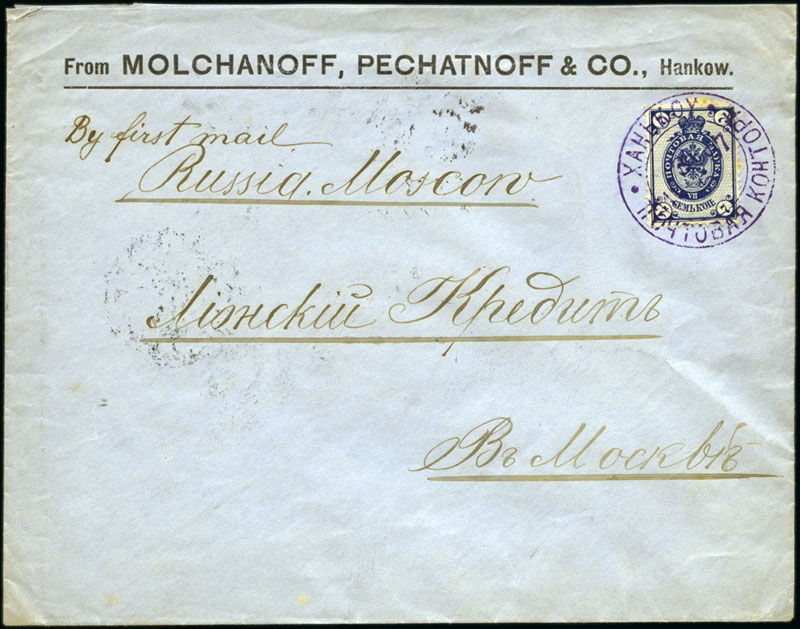
\includegraphics[width=.95\textwidth]{../russian-post-offices-in-china/10108.jpg}
\caption{10108	HANKOW: 1897 Cover to Moscow with Arms 7k tied by double ring 
Hankow 31.5.97 cds in violet (T\&S type 1), with further strike on reverse 
along with Odessa and Moscow cds.
The earliest recorded cover from the Russian P.O. in Hankow.
\euro 4,000.00} 
\end{figure} 

\begin{figure}[htbp]
\centering
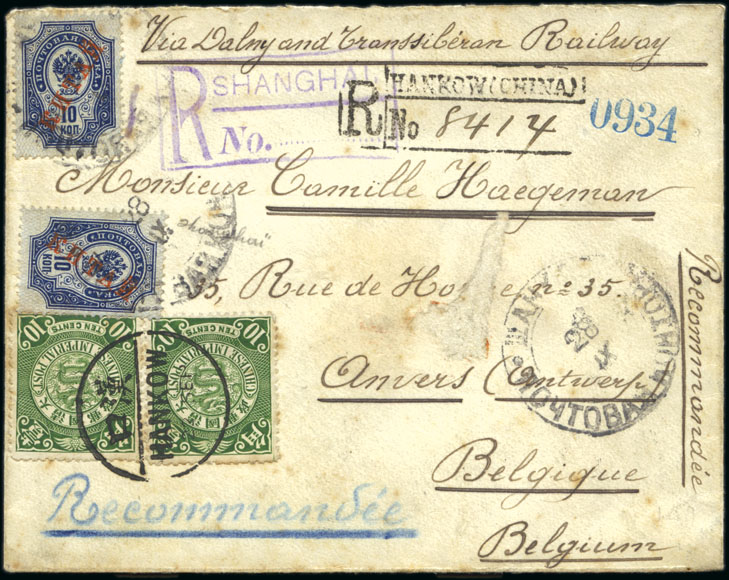
\includegraphics[width=.95\textwidth]{../russian-post-offices-in-china/10109.jpg}
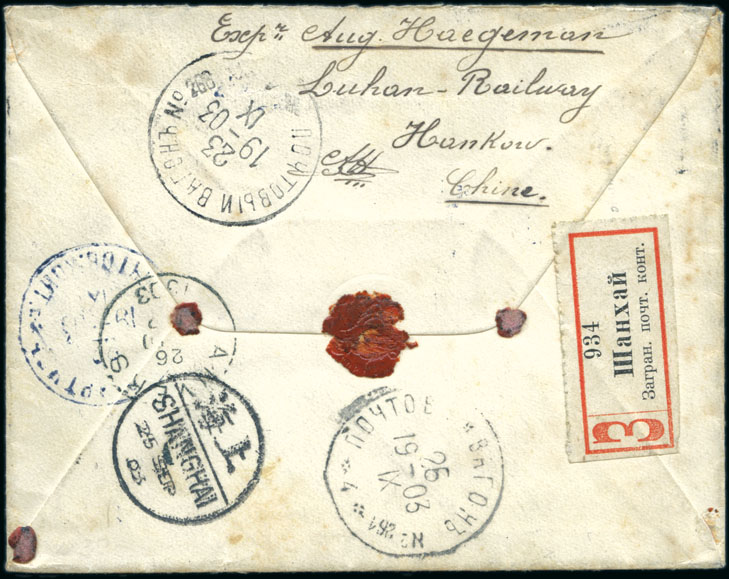
\includegraphics[width=.95\textwidth]{../russian-post-offices-in-china/10109-1.jpg}
\caption{ 
10109 HANKOW: 1903 Cover registered to Belgium, franked initially with 
two China 10c Dragons tied by Hankow bilingual cds, with boxed registration 
hs adjacent, sent to Shanghai where it was passed to the Russian P.O. 
and franked with two "KITAI" 10k tied by Shanghai 28.9.03 cds (T\&S type 1), 
with boxed reg'n hs and label (reverse), transits of Port Arthur, 
"Postal Wagon No.266 / 4" (Port Arthur-Harbin) and "Postal Wagon 261 / 4" 
(Manchuli-Harbin), slightly soiled, rare two country franking
\euro 2,000.00 
} 
\end{figure} 

\begin{figure}[htbp]
\centering
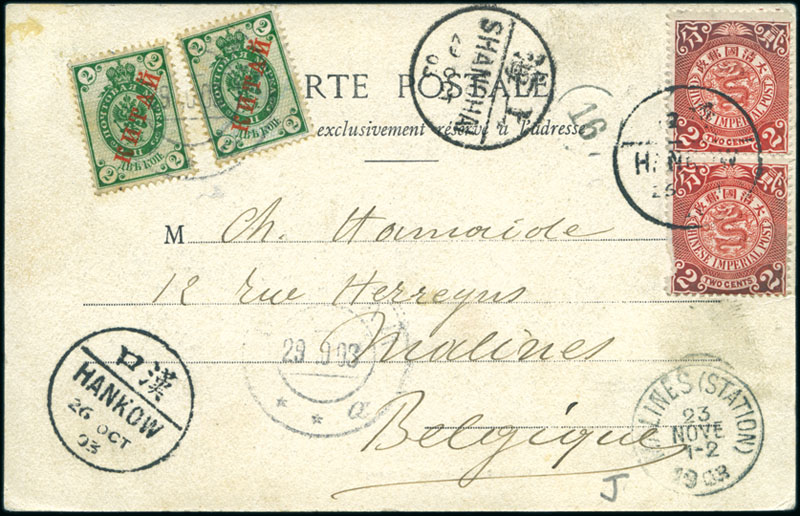
\includegraphics[width=.95\textwidth]{../russian-post-offices-in-china/10110.jpg}
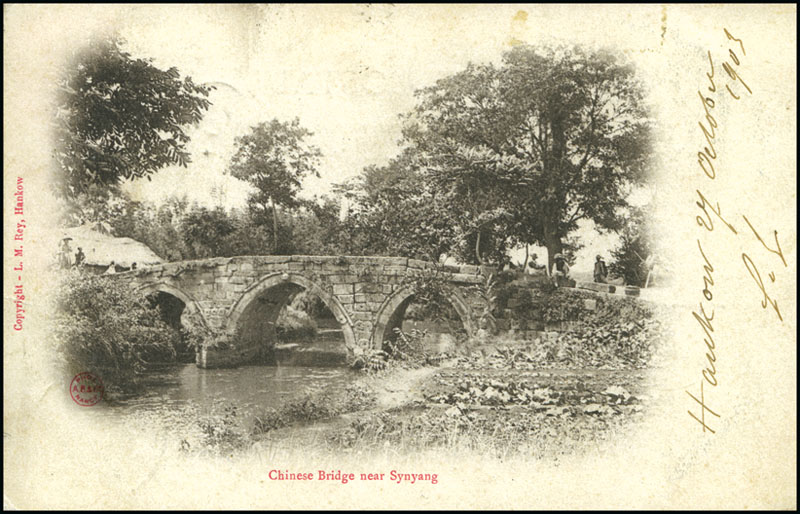
\includegraphics[width=.95\textwidth]{../russian-post-offices-in-china/10110-1.jpg}
\caption{ 
10110	HANKOW: 1903 Picture postcard to Belgium with China 2c Dragon in 
vertical pair tied by bilingual Hankow 26.10.03 cds, sent to Shanghai 
where it was transferred to the Russian P.O. and franked with two "KITAI" 
2k tied by Shanghai cds (T\&S type 3), Maillines (Station) arrival, fine

Note: Although a Russian P.O.had existed at Hankow since 1896, 
it was frequently by-passed in preference to the Chinese P.O., 
which had a quicker service down the River Yangtze to Shanghai.
\euro 700.00
} 
\end{figure} 

\begin{figure}[htbp]
\centering
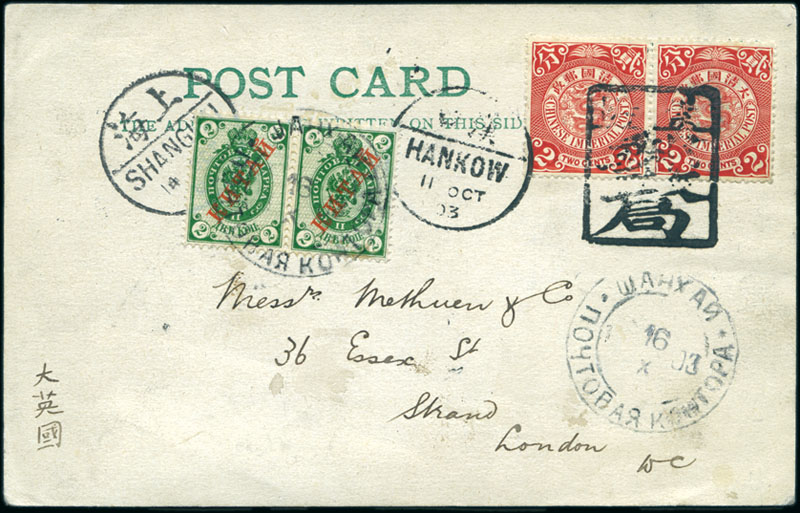
\includegraphics[width=.95\textwidth]{../russian-post-offices-in-china/10111.jpg}
\caption{ 
10111HANKOW: 1903 Postcard from the Wesleyan Mission to England with China 2c 
Dragon pair tied by boxed local cancel, sent to Shanghai where it was transferred 
to the Russian P.O. and franked with "KITAI" 2k pair tied by 
Shanghai cds (T\&S type 1), Moscow bs, fine

Note: Although a Russian P.O.had existed at Hankow since 1896, 
it was frequently by-passed in preference to the Chinese P.O., 
which had a quicker service down the River Yangtze to Shanghai.
\euro 800.00 
} 
\end{figure} 

\subsection{Newspaper Wrapper}
\begin{figure}[htbp]
\centering
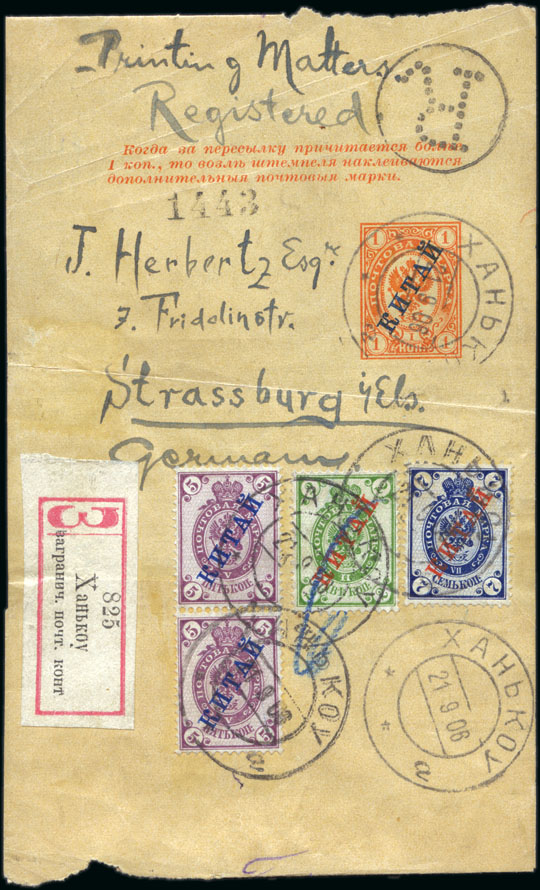
\includegraphics[width=.95\textwidth]{../russian-post-offices-in-china/10112.jpg}
\caption{ 
10112HANKOW: 1906 "KITAI" 1k newspaper wrapper registered to Germany, 
uprated with "KITAI" 2k, 5k (2) and 7k, all cancelled by Hankow 21.9.06 cds 
(T\&S type 2A), with reg'd label in Cyrillic and encircled "dotted R" hs, 
opened for display, a rare use of this postal stationery.
\euro 400.00 
} 
\end{figure} 

\subsection{Registered Envelope}
\begin{figure}[htbp]
\centering
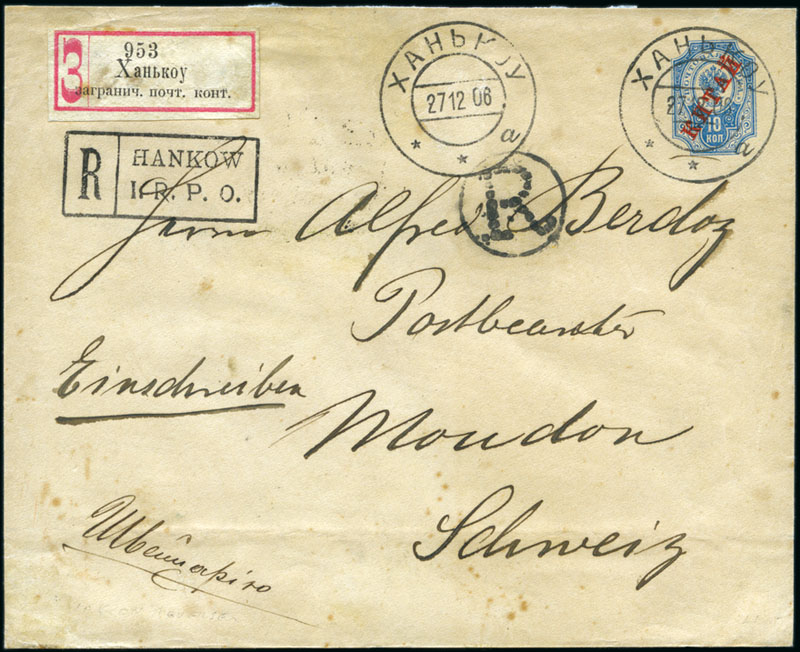
\includegraphics[width=.95\textwidth]{../russian-post-offices-in-china/10113.jpg}
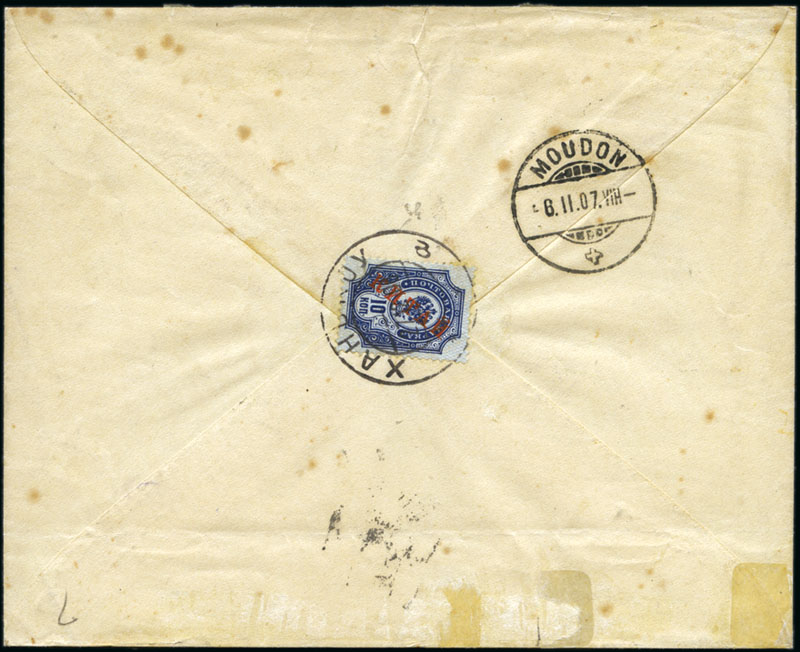
\includegraphics[width=.95\textwidth]{../russian-post-offices-in-china/10113-1.jpg}
\caption{ 
10113	HANKOW: "KITAI" 10k postal stationery envelope registered to Switzerland, 
uprated on the reverse with "KITAI" 10k, both cancelled by Hankow 27.12.06 cds 
(T\&S type 2a), with boxed reg'n cachet in English and reg'd label 
in Cyrillic, along with encircled "dotted R", minor fox spots, a 
scarce use of postal staionery and very rare registered handstamp
\euro 500.00 
} 
\end{figure} 



  
  
  
  
  
  
  
  
  
  
  
  
  
  
  
                